% Created 2016-02-05 Fri 09:42
\documentclass{scrartcl}
\usepackage[utf8]{inputenc}
\usepackage[T1]{fontenc}
\usepackage{fixltx2e}
\usepackage{graphicx}
\usepackage{longtable}
\usepackage{float}
\usepackage{wrapfig}
\usepackage{soul}
\usepackage{textcomp}
\usepackage{marvosym}
\usepackage{wasysym}
\usepackage{latexsym}
\usepackage{amssymb}
\usepackage{hyperref}
\tolerance=1000
\usepackage{khpreamble}
\providecommand{\alert}[1]{\textbf{#1}}

\title{Computerized control - homework 2}
\author{Kjartan Halvorsen}
\date{Due 2016-02-05}
\hypersetup{
  pdfkeywords={},
  pdfsubject={},
  pdfcreator={Emacs Org-mode version 7.9.3f}}

\begin{document}

\maketitle



\section*{Exercises}
\label{sec-1}
\subsection*{Sample the continuous-time transfer function}
\label{sec-1-1}

   Consider the harmonic oscillator with transfer function 
   \begin{equation}
    G(s) = \frac{\omega^2}{s^2 + \omega^2}.
    \label{eq:contsys}
    \end{equation}


   \textbf{Compute the pulse-transfer function} by sampling the transfer function $G(s)$. 
\subsection*{Simulation of the continuous- and discrete-time harmonic oscillator}
\label{sec-1-2}

Use matlab's control toolbox or the \href{http://python-control.sourceforge.net/}{python control module}  to simulate the system and verify your calculations. 
\subsubsection*{Define systems}
\label{sec-1-2-1}

First, define the continuous-time system in \eqref{eq:contsys}

\begin{verbatim}
omega = 1; % Just a suggestion
h = 0.2/omega; % Completely undamped system. This gives about 30 samples per period 
sys_c = tf([omega^2],[1 0 omega^2])
\end{verbatim}
Sample the system using the function \texttt{c2d}

\begin{verbatim}
sys_c2d = c2d(sys_c, h)
\end{verbatim}
Define the discrete-time system you calculated in the first part of the homework

\begin{verbatim}
den = [1 a1 a2];
num = [b1 b2];
sys_d = tf(num, den, h)
\end{verbatim}
\textbf{Verify that the two discrete-time systems} \texttt{sys\_c2d} \textbf{and} \texttt{sys\_d} \textbf{are identical.}
\subsubsection*{Simulate step responses}
\label{sec-1-2-2}

Simulate for 4 complete periods 

\begin{verbatim}
Tc = linspace(0, 4*(2*pi/omega), 800);
[yc,tc] = step(sys_c, Tc);

Td = h*(0:120);
[yd,td] = step(sys_d, Td);

figure()
clf
plot(tc,yc)
hold on
plot(td,yd, 'r*')
\end{verbatim}

\textbf{Verify that the step response of the discrete-time system is exactly equal to that of the continuous-time system at the sampling instants. Explain why this is so!}
\subsubsection*{Compute the discrete step response yourself}
\label{sec-1-2-3}

    Write some lines of code that solves the difference equation
    \[ y(k+2) = -a_1y(k+1) - a_2y(k) + b_1u(k+1) + b_2u(k) \]
    for the harmonic oscillator. 
   Use the initial state \(y(-1)=y(0)=0\) and compute the response to a step sequence 
    \[ u(k) = \begin{cases} 1, & k \ge 0\\ 0, & \text{otherwise} \end{cases}.\]
    Verify that your solution is the same as when using the \texttt{step} function in the previous exercise in this homework.
 
\section*{Solutions}
\label{sec-2}
\subsection*{Sampling the transfer function}
\label{sec-2-1}

\begin{enumerate}
\item Calculate the step response
      \begin{equation*}
       \begin{split} 
         Y(s) &= G(s)\frac{1}{s} = \frac{\omega^2}{(s^2 + \omega^2)s}\\
              &= \frac{1}{s} - \frac{s}{s^2 + \omega^2}.
       \end{split}
      \end{equation*}
\item Transform to time domain (using transform table) 
      \[ y(t) = u(t) - u(t) \cos \omega t \]
\item Calculate z-transform of sampled output 
      \begin{equation*}
       \begin{split} 
        Y(z) &= \ztrf{y(kh)} = \ztrf{u(kh) - u(kh)\cos(\omega k h)}\\
             &= \ztrf{u(k)} - \ztrf{u(k)\cos(\omega hk)}\\
             &= \frac{z}{z-1} - \frac{z(z-\cos(\omega h))}{z^2 -2\cos(\omega h)z +1}
       \end{split}
      \end{equation*}
\item Divide by the z-transform of the step input
       \begin{equation*}
        \begin{split}
         H(z) &= \frac{Y(z)}{U(z)} = \frac{z-1}{z} \Big( \frac{z}{z-1} - \frac{z(z-\cos(\omega h))}{z^2 -2\cos(\omega h)z +1}\Big)\\
              &= 1 - \frac{(z-1)(z-\cos(\omega h))}{z^2 -2\cos(\omega h)z +1}\\
              &= \frac{z^2 - 2\cos(\omega h)z + 1 - z^2 +\cos(\omega h)z + z - \cos(\omega h)}{z^2 - 2\cos(\omega h)z + 1}\\
              &= \frac{\big(1-\cos(\omega H)\big)z + 1-\cos(\omega h)}{z^2 - 2\cos(\omega h)z + 1}.
        \end{split}
       \end{equation*}
\end{enumerate}
\subsection*{Simulations}
\label{sec-2-2}

   The code that is provided does most of the job. You just have to define the numerator and denominator of the discrete-time system from the sampled model you obtained:

\begin{verbatim}
a1 = -2*cos(omega*h);
a2 = 1;
b1 = 1-cos(omega*h);
b2 = b1;

den = [1 a1 a2];
num = [0 b1 b2];
sys_d = tf(num, den, h)
\end{verbatim}
\subsection*{Own code for simulating system response}
\label{sec-2-3}

   There are many ways to do this. Here is one

\begin{verbatim}
% Calculate the step response by hand
N = 120;
u = ones(N,1);
y = nan(N,1);
% Pad with two zeros at beginning, corresponding to u(-2), u(-1), y(-2) and
% y(-1)
u = [zeros(2,1); u];
y = [zeros(2,1); y];

for kplustwo = 3:N
    y(kplustwo) = -a1*y(kplustwo-1) -a2*y(kplustwo-2) + b1*u(kplustwo-1) + b2*u(kplustwo-2);
end

yd2 = y(3:end);
plot(td,yd2, 'ko', 'markersize', 14)
legend('Continous model', 'Discrete model', 'Own simulation')
\end{verbatim}

\begin{center}
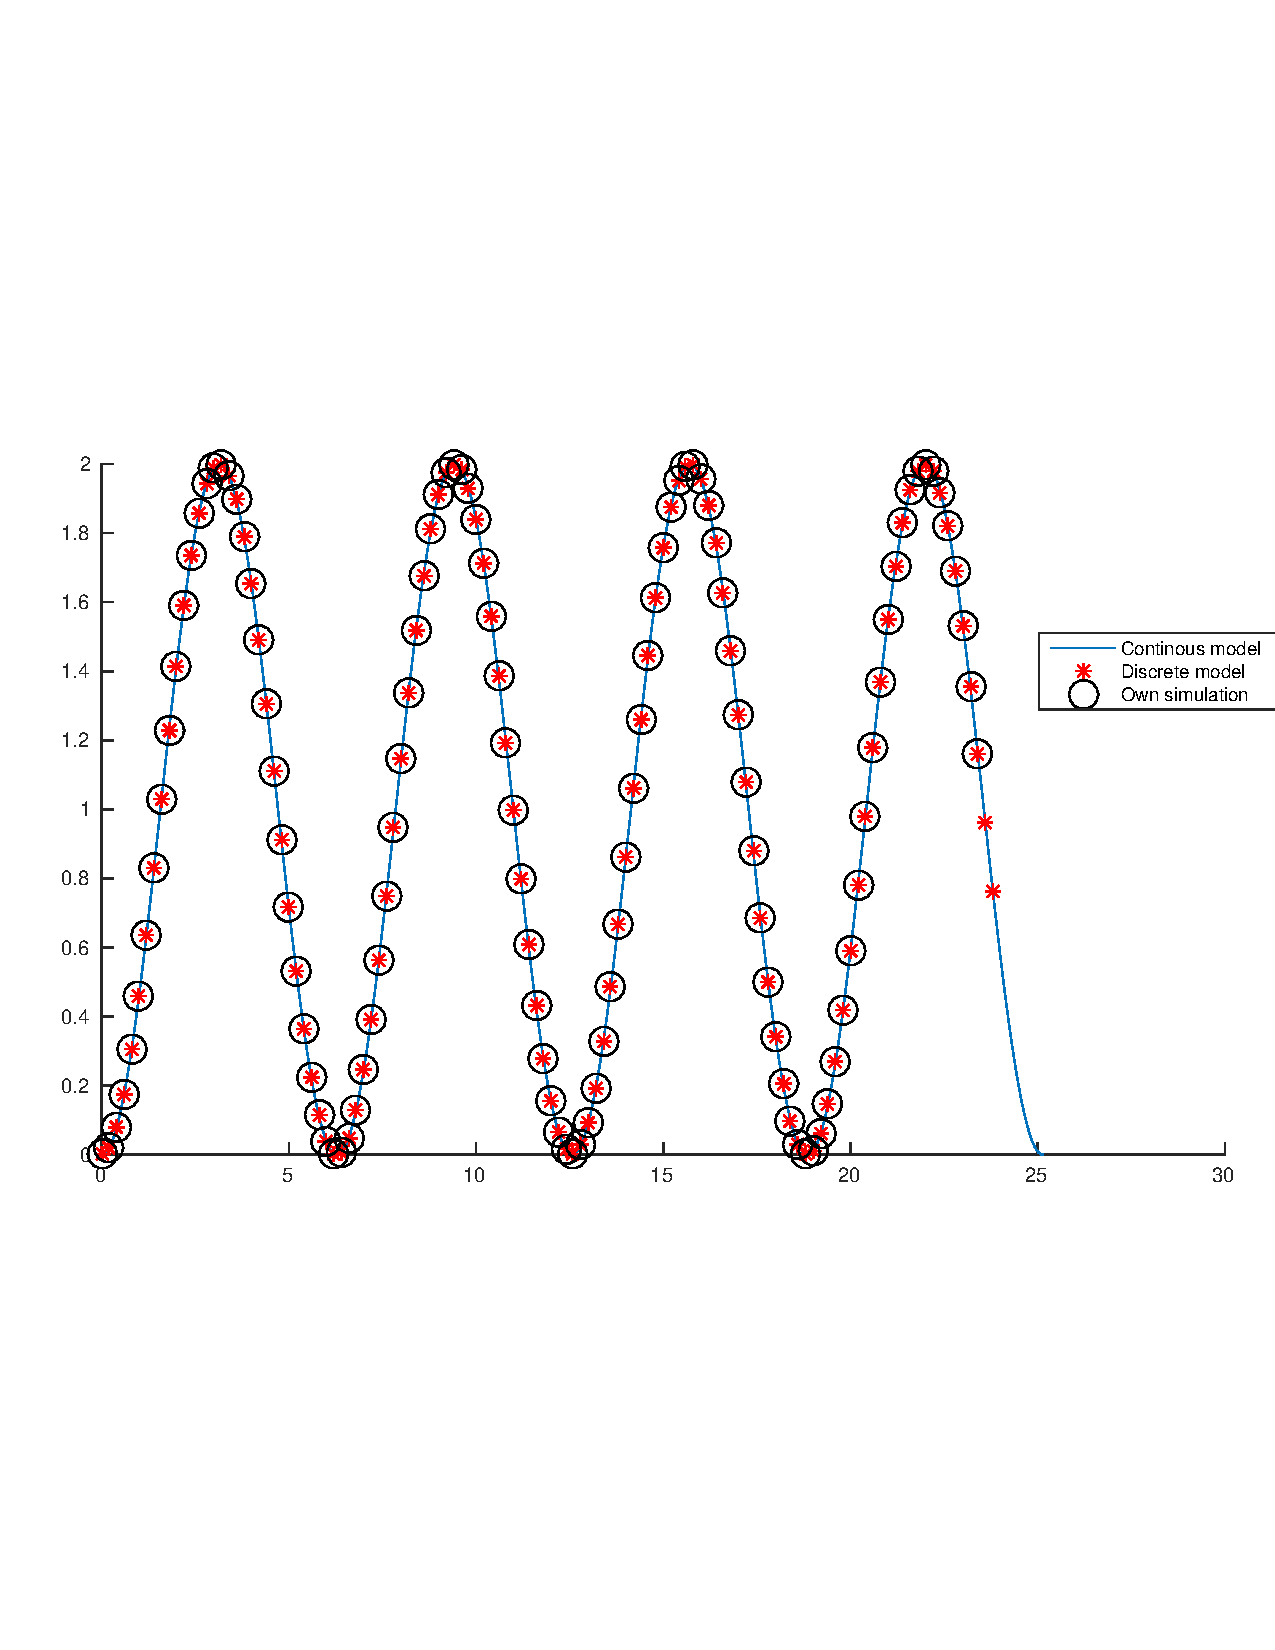
\includegraphics[width=0.7\linewidth]{hw2-spring16-sim}
\end{center}

\end{document}
